%%%
%%%
%%%
%% Bu tez TNKÜ FBE için İTÜ'ne ait itutez.cls baz alınarak hazırlanmıştır.
%%% İTÜtezin bazı/birçok özelliği kullanılmamaktadır.

% ---------------------------------------------------------------- %
%                     LATEX Tez Sablonu		                   %
%                                                                  %
%		         Surum 1.5.1                               %
% ---------------------------------------------------------------- %

% ---------------------------------------------------------------- %
% ITU Bilisim Enstitusu tarafindan hazirlanmistir.	           %
%                                                                  %
% İTÜ Ayazağa Kampüsü, Bilişim Enstitüsü Binası                    %
% Maslak-34469, İstanbul 	                                   %
% http://www.be.itu.edu.tr                                         %
% ---------------------------------------------------------------- %

\documentclass[tekyonlu,turkce,yukseklisans,karton,fenbilimleri]{tnkutez}
% ---------------------------------------------------------------- %
% Komutlarda buyuk ve kucuk harf ayrimina ozen gostermek           %
% gereklidir. Ornegin argumanin {\"O\u{g}\-ren\-ci Ad{\i}}{SOYADI} %
% yapisinda olmasi demek, adlarda ilk harflerin buyuk ve           %
% digerlerinin kucuk, soyadinda ise butun harflerin buyuk olmasi   %
% gerektigi anlamina gelmektedir.				   %
% ---------------------------------------------------------------- %

           


\tolerance=1
\emergencystretch=\maxdimen
\hyphenpenalty=10000
\hbadness=10000

\usepackage{adjustbox}
\usepackage{graphicx}

% ---------------------------------------------------------------- %
% Sadece Ad SOYAD yazilmalidir. Unvan yazilmamalidir.              %
% ---------------------------------------------------------------- %
\yazar{Ad}{SOYAD} 
\ogrencino{ }

% ---------------------------------------------------------------- %
% Kullanmayacaginiz yapilarin ayirac aralarini bos birakiniz.      %
% Ornek: \unvan{}                                                  %
% ---------------------------------------------------------------- %
%MESLEK YAZILACAK
\unvan{Meslek}
 
% ---------------------------------------------------------------- %
% Asagidaki yapilarda birinci oge Turkce, ikinci oge Ingilizce     %
% yapiyi olusturmak icindir.	                                   %
% ---------------------------------------------------------------- %

% ---------------------------------------------------------------- %
% Sozcuklerin ilk harfleri buyuk, diger harfler kucuk yazilacak.   %
% ---------------------------------------------------------------- %
\anabilimdali{AAA Anabilim Dal{\i}}{Department of AAA}
\programi{}{}


\tarih{TEKİRDAĞ-2019}{TEKİRDAĞ-2019} 
\tarihKucuk{2019}{2019}
\tarihAyYil{Mart 2019}{March 2019}
% ---------------------------------------------------------------- %
% Danisman, baslik ve tez tarihi bilgileri icin asagidaki yapi     %
% kullanilmaktadir.						   %
% ---------------------------------------------------------------- %

% ---------------------------------------------------------------- %
% Danisman bilgisi %						
% ---------------------------------------------------------------- %
\tezyoneticisi{Prof. Dr. Ad SOYAD}{Tekirdağ Namık Kemal Üniversitesi}   


%Tez başlığı %
\baslik{TEZ BAŞLIĞI BURAYA GELİR}{GEREKLİ İSE İKİNCİ SATIR}{GEREKLİ İSE ÜÇÜNCÜ SATIR, ÜÇ SATIRA SIĞDIRINIZ}

\title{THESIS TITLE HERE}{SECOND LINE IF NECESSARY}{THIRD LINE IF NECESSARY, FIT TITLE IN THREE LINES}

% ---------------------------------------------------------------- %
% ---------------------------------------------------------------- %
\tezvermetarih{15.04.2019}{Nisan 2019} 
\tezsavunmatarih{15.03.2019}{Mart 2015}

% ---------------------------------------------------------------- %
% Esdanisman ve juri bilgileri asagidadir. Kullanmayacaginiz satiri%
% tumuyle silmeyiniz. Argumanini bos birakiniz.                    %
% Ornek: \esdanismani{}{} 					   %
% ---------------------------------------------------------------- %

\esdanismani{Prof. Dr. Ad{\i} SOYADI}{}  
% es danışman yok ise aşağıdaki gibi bırakıyoruz 
%\esdanismani{}{}   

\juriBir{Prof. Dr. Ad{\i} SOYADI}{}

\juriIki{Prof. Dr. Ad{\i} SOYADI}{}

\juriUc{Prof. Dr. Ad{\i} SOYADI}{}

\juriDort{Prof. Dr. Ad{\i} SOYADI}{}

\juriBes{Prof. Dr. Ad{\i} SOYADI}{}


\enstitumuduru{Doç. Dr. Bahar UYMAZ}{}

%%%% ONEMLİ aşağıdaki iki referans stilinden birini seçmelisiniz.

\input defs-alfabetik-apa-stili.tex
%\input defs-numerik-ieee-stili.tex


% bib dosyanız olmalı. Mendeley gibi programlar bu dosyaları 
% otomatik üretirler.
\addbibresource{refs.bib}                     

% ---------------------------------------------------------------- %
% Ithaf sayfasinda bulunacak tumceler icin kullanilabilecek        %
% yapi asagidadir. Ithaf sayfasi bulunmayacaksa argumani(ayiraclar %
% arasini) bos birakiniz.					   %
% ---------------------------------------------------------------- %
\ithaf{}

% ---------------------------------------------------------------- %
% Proje sayfasinda bulunacak tumceler icin kullanilabilecek        %
% yapi asagidadir. Proje sayfasi bulunmayacaksa argumani(ayiraclar %
% arasini) bos birakiniz.					   %
% ---------------------------------------------------------------- %
% proje
\proje{Bu tez .................... (TÜBİTAK / SANTEZ / NKÜBAP vb.) .................. tarafından ................................................................... numaralı proje ile desteklenmiştir. }

% ---------------------------------------------------------------- %
% Asagida belirtilen tex uzantili dosyalarin icerigi		   %
% olusturulmalidir.						   %
% ---------------------------------------------------------------- %

\ozet{\input ozet.tex}
\summary{\input summary.tex}  
\kisaltmalistesi{\input simge_ve_kisaltmalar.tex}
\onsoz{\input tesekkur.tex}             
        
\begin{document}


%
% İsterseniz aşağıdaki tez içeriğini bölümlere ayırabilirsiniz.
% ---------------------------------------------------------------- %
% Asagida belirtilen tex uzantili dosyalarin icerigi		   %
% olusturabilirsiniz. Tezin butun bolumlerine karsilik gelen girdi   %
% satirlari belirtilmelidir. Eger tezinizde daha az bolum varsa,   %
% karsilik gelen \input bolumx.tex satirlari silinmelidir.            %
% ---------------------------------------------------------------- %
%\input bolum1.tex
%\input bolum2.tex
%\input bolum3.tex
%\input bolum4.tex



% tez baslar
%%%%%%%%%%%%%%%%%%%%%%%%%%%%%%%%%%%%%%%%%%%%%%

\chapter{GİRİŞ}
\hspace{1.25cm}Bu bölümde tez konusuyla ilgili olarak hazırlayıcı bilgiler verildikten sonra araştırmanın amacı ve kapsamı açıkça belirtilmelidir. Ayrıca, eğer tez konusu ile ilgili olarak söz edilmek istenen önceki çalışmalar varsa, bunlar da GİRİŞ bölümü içinde verilebilir. 

Eğer tez çalışmasında ve yazımında olağandışı ve/veya tartışmalı bir adlandırma, sınıflama ve kavram kullanılmışsa, bunların açıklaması yine GİRİŞ bölümünde verilmelidir. 

\section{İkinci Dereceden Başlık}
Tezin herhangi bir sayfasında metnin içinde yazılması halinde konuyu dağıtıcı ve okumada sürekliliği engelleyici nitelikteki çok kısa ve öz açıklamalar birkaç satır halinde aynı sayfanın altına dipnot olarak verilebilir. Dipnotlar sayfa içindeki ana metinden iki aralık bırakıldıktan sonra, soldan sağa bir çizgi ile ayrılmalıdır. Sayfanın alt kenarında bırakılması gereken boşluğa kesinlikle taşmamalıdır.

Yazılan ilk dipnotta\footnote{Dipnotlar bu örnekteki gibi yazılmalı.}   Latex kaynak dosyasında (tezim.tex) gösterildiği gibi kullanılmalıdır. İkinci\footnote{İkinci dipnot. İkinci ve sonraki dipnot metinleri}, üçüncü\footnote{İkinci ve sonraki dipnot metinleri.} ve sonraki dipnotlarda ise satır aralıkları tek satır olarak ayarlanmalıdır. 

Dipnot çizgisi ile dipnot numarası arasında bir aralık boşluk bırakılmalıdır. Dipnot simgesi Arabic rakam olarak seçilmeli ve dipnot simgesinden sonra bir boşluk bulunmalıdır. Dipnotun açıklaması bir satır aralığı ile yazılmalı ve 8 punto kullanılmalıdır. Dipnotlar her sayfa içinde belirme sırasına göre "1" den başlayarak numaralandırılmalı ve dipnot açıklaması mutlaka değinilen sayfada yer almalıdır. 

\subsection{Sayıların Yazılışı}
Bir zorunluluk olmadıkça cümle rakamla başlamamalıdır.

Dört veya daha çok basamaklı sayılar sondan sayılmak üzere üçlü gruplara ayrılarak yazılmalı ve aralarına nokta konulmalıdır:

Örnek: 3.822 (Üç bin sekiz yüz yirmi iki)

196.995 (Yüz doksan altı bin dokuz yüz doksan beş)

81.250.124 (Seksen bir milyon iki yüz elli bin yüz yirmi dört )

Dört veya daha çok basamaklı sayıların kolay okunabilmesi amacıyla içinde geçen bin, milyon, milyar ve trilyon sözleri harfle yazılabilir.

Örnek: 12 trilyon 300 milyar 245 milyon 595 bin (12.300.245.595.000)


\subsubsection{Kesirlerin yazılışı}
Sayılarda kesirler virgülle ayrılmalıdır.

Örnek: 12,7 (12 tam, onda 7)

Bayağı kesirlere getirilecek ekler alttaki sayı esas alınarak yazılmalıdır.

Örnek: 2/3’ü (iki bölü üçü), 1/7’si (bir bölü yedisi).

Birbirini takip eden ondalık sayılar noktalı virgül ";" ile ayrılmalıdır.

Örnek: 12,7; 9,45; 2,11 vb.

Yüzde ve binde işaretleri yazılırken sayılarla işaret arasında boşluk bırakılmamalıdır.

Örnek: \%25, \textperthousand 50 vb.


\subsection{Çizelge Örneği}
Tezin yazımında kullanılabilecek iki tip çizelge aşağıda verilmiştir. Çizelge ve numarası kalın yazılmalıdır. 

\begin{table}[!t]
	\caption{Çizelge başlığı cümle sonuna nokta konulmadan iki yana yaslı olarak bölüm numarası ile birlikte yazılmalıdır}
	%\begin{adjustbox}{width=1\textwidth}
	\begin{tabular}{L{3cm}L{3cm}L{3cm}L{3cm}}
		\hline\hline
		Başlık&Başlık&Başlık&Başlık\\\hline
		A&&&\\
		B&&&\\
		C&&&\\
		\hline\hline
	\end{tabular}
	%\end{adjustbox}
	\vspace{24pt}
\end{table}


\begin{table}[!t]
	\caption{Örnek tablo 2}
	\begin{tabular}{L{3cm}L{3cm}L{3cm}L{3cm}}
		\hline
		Başlık&Başlık&Başlık&Başlık\\\hline
		A&&&\\
		B&&&\\
		C&&&\\
		\hline
	\end{tabular}
	\vspace{24pt}	
\end{table}

Çizelgelerden sonra yazılacak paragrafın çizelge ile arasında 24 nk boşluk olmalıdır. 

\subsection{Şekil Örneği}
Şekillerin başlık yazısı ilgili yere yazılmalıdır.

\begin{figure}[!h]
	%\centering
	
\includegraphics[width=0.2\linewidth]{sekiller/nku_logo}
	\caption{Şekil başlığı cümle sonuna nokta konulmadan iki yana yaslı olarak bölüm numarası ile birlikte yazılmalıdır}
	\label{fig:nkulogo}
	\vspace{24pt}
\end{figure}

Şekillerden sonra yazılan paragraflar ile şekil yazıları arasındaki boşluk 24 nk olmalıdır. 

\begin{figure}
	%\centering
	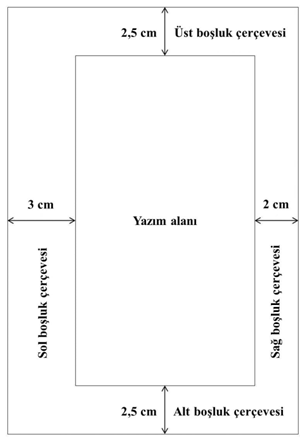
\includegraphics[width=0.2\linewidth]{sekiller/sekil}
	\caption{Örnek şekil yazısı 2}
	\label{fig:sekil}
	\vspace{24pt}
\end{figure}

\subsection{Denklem Örnekleri}
Denklem yazarken denklemler sayfayı ortalamış, numarası da sayfanın sağına yaslanmış olmalıdır. Bunu sağlayabilmek için kenarlığı olmayan bir tablo kullanılabilir.
\begin{equation}
f(x)=a_0+\sum_{n=1}^{\infty}\left(a_n\cos\frac{n\pi x}{L}+b_n\sin\frac{n\pi x}{L}\right)
\end{equation}
\begin{equation}
a^2+b^2=c^2
\end{equation}

Denklemlerden sonra paragraf buradan başlar.

\subsection{Madde İşaretleri ve Numaralandırma}
Madde işaretleri 1,25 cm içeriden ve 1,75 sekme durak yeri ile yapılmalıdır. 
\begin{itemize}
	\setlength{\itemindent}{1.25cm}
	\item Örnek işaretlenmiş metin 1
	\item Örnek işaretlenmiş metin 2
	\item Örnek işaretlenmiş metin 3
	\item Örnek işaretlenmiş metin 4
\end{itemize}

Madde numaralandırma 1,25 cm içeriden ve 1,75 sekme durak yeri ile yapılmalıdır.
\begin{enumerate}
	\setlength{\itemindent}{1.25cm}
	\item Örnek numaralandırılmış metin 1
	\item Örnek numaralandırılmış metin 2
	\item Örnek numaralandırılmış metin 3
	\item Örnek numaralandırılmış metin 4
\end{enumerate}


\section{Latex'te Referans verme}

Eğer apa stilini kullanıyorsanız parantez içi kullanım için \verb|\parencite{}|, cümle içi kullanım için ise \verb|\citet{}| olarak referans vermelisiniz.

Eğer IEEE stili kullanıyorsanız sadece \verb|\cite{}| olarak referans vermelisiniz.

\citet{Sakamoto2005}, \parencite{Sakamoto2005}
\cite{Thompson2014}

\chapter{İKİNCİ BÖLÜM}
\chapter{ÜÇÜNCÜ BÖLÜM}
\chapter{DÖRDÜNCÜ BÖLÜM}
\chapter{BEŞİNCİ BÖLÜM}


%%%%%%%%%%%%%%%%%%%%%%%%%%%%%%%%%%%%%%%%%%%%%%%
%tez biter



% ---------------------------------------------------------------- %
% Bibtex veritabani biceminde olmasi gereken library.bib dosyasina     %
% tezin referanslari yerlestirilmeli, bu referanslara, tez         %
% icerisinde \cite{} \citet{} \parencite{} komutları ile basvuru yapilmalidir.                %
% ---------------------------------------------------------------- %
\newpage
\addtocontents{toc}{\addvspace{-10pt}}
\addcontentsline{toc}{chapter}{\bf{KAYNAKLAR}}
\printbibliography[title=\normalsize{KAYNAKLAR}]

% ---------------------------------------------------------------- %
% Ekler icin asagida belirtilen tex uzantili dosyalar 		   %
% olusturulmali, eger ek kullanilmayacaksa, karsilik gelen         %
% satirlar silinmelidir.                                           %
% ---------------------------------------------------------------- %
%\eklerkapak{}
%\input eklerkapak.tex  

% ---------------------------------------------------------------- %
% Ek icin bolum ayari. \eklerbolum{x} x bolumlu olusturur. Bu olgu,% 
% tablo ve sekillerin adreslenmesinde bu baglamda kullanilir. A    %
% ile baslamak icin \eklerbolum{0} yazilmalidir.                   %
% ---------------------------------------------------------------- %
%\eklerbolum{0}
%\input ekler.tex

% ---------------------------------------------------------------- %
% Ozgecmis ile ilgili dosya adi asagida belirtilmistir.            %
% ---------------------------------------------------------------- %
\ozgecmis{\input ozgecmis.tex}
\end{document}                      

% ---------------------------------------------------------------- %
% LATEX Sablonu ile ilgili iletisim icin: iletisim@be.itu.edu.tr   %
% ---------------------------------------------------------------- %
